\documentclass[14pt]{article}

\usepackage[utf8x]{inputenc}
\usepackage[russian]{babel}
\usepackage{graphicx}
\graphicspath{{images/}}
\DeclareGraphicsExtensions{.pdf,.png,.jpg}

\usepackage{amsmath}
\usepackage{pgfplots}

\usepackage{geometry} % Меняем поля страницы
\geometry{left=2cm}% левое поле
\geometry{right=1.5cm}% правое поле
\geometry{top=2cm}% верхнее поле
\geometry{bottom=2cm}% нижнее поле

\renewcommand{\theenumi}{\arabic{enumi}}
\renewcommand{\labelenumi}{\arabic{enumi}}
\renewcommand{\theenumii}{.\arabic{enumii}}
\renewcommand{\labelenumii}{\arabic{enumi}.\arabic{enumii}.}
\renewcommand{\theenumiii}{.\arabic{enumiii}}
\renewcommand{\labelenumiii}{\arabic{enumi}.\arabic{enumii}.\arabic{enumiii}.}

\begin{document}
\begin{titlepage}
	\begin{center}
		\fontsize{18pt}{20pt}\selectfont
		\textbf{Работа 4.4.1.}	
	
		\vspace{5cm}
		\fontsize{24pt}{25pt}\selectfont
		Изучение амплитудной решетки
	\end{center}
	\begin{flushright}
		\fontsize{18pt}{20pt}\selectfont
		\vspace{14cm}
		\hspace{-3cm}
		\textit{Корнеев Е.С.}
	\end{flushright}		
\end{titlepage}

\begin{center}
	\fontsize{16pt}{18pt}\selectfont
	Изучение амплитудной решетки
\end{center}


\fontsize{14pt}{16pt}\selectfont

\vspace{0.5cm}
\textbf{Оборудование:} гониометр, ртутная лампа, амплитудная решетка, призменный уголковый отражатель, щель с микрометрическим винтом.

\vspace{1cm}

В данной работе мы отъюстируем гониометр, исследуем спектр ртутной лампы в $\pm 1$ порядках и дисперсию ретётки в разных порядках, определим период и спектральные характеристики решётки, а также оценим влияние ширины пучка на разретающую способность.

Предварительно проведем качественные наблюдения спектра: держа решётку в руке и глядя сквозь неё на узкий источник света, найдём спектр нулевого порядка -- ахроматическое (белое) изображение источника.

Поворачивая решётку вокруг вертикальной оси, рассмотрим спектры положительных и отрицательных порядков.

Определим, в каких порядках спектры начинают перекрываться, и оценим дисперсионную область решётки.

\vspace{1cm}
\textbf{I. Установка решётки}

Необходимость дополнительной настройки столика с решёткой связана с тем, что плоскость решётки может быть не перпендикулярна её основанию, и тогда при повороте зрительной трубы спектры дальних порядков могут уйти из поля зрения.

Настроим зрительную трубу на наблюдение входной щели коллиматора. Начало отсчёта угла примем равным $180^\circ$, вертикальный размер изображения щели занимет менее четверти поля зрения трубы.

Установим решётку на столике так, чтобы её плоскость была параллельна одному из винтов 8 и перпендикулярна оси коллиматора. Вращая только верхнюю часть столика (винт 26 закреплён, чтобы не сбилась настройка нуля), найдем ахроматическое (белое) изображение щели коллиматора -- спектр нулевого порядка.

Винтом 8, перпендикулярным плоскости решётки, установим изображение щели на центр поля зрения.

\begin{figure}[h!]
	\center{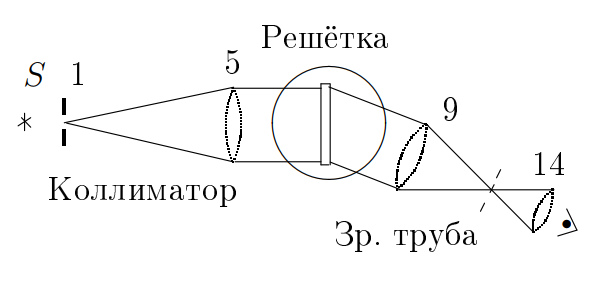
\includegraphics[width = 10cm]{1}}
	\caption{Схема установки}
	\label{fig:image}
\end{figure}

Отводя алидаду в сторону от коллиматора, найдем в трубе спектр самого дальнего порядка, и винтом 8, параллельным плоскости ретётки, снова приведем изображение щели к центру.

Вернемся к ахроматическому изображению щели и проверим результат. При необходимости снова подстроим столик винтом, перпендикулярным плоскости решётки. Повторяя процедуру, методом последовательных приближений добьемся того, чтобы при повороте трубы изображение щели и спектр уходили не больше, чем на треть радиуса поля зрения.

\vspace{1cm}
\textbf{II. Исследование спектра ртутной лампы}

Подберем ширину входной щели так, чтобы ширина жёлтой спектральной линии была чуть больше (1.5-2 раза) промежутка между линиями двойного штриха окуляра зрительной трубы.

Установим высоту щели, удобную для измерений. Перед началом измерений убедимся в справедливости формулы
$$
	d\sin\varphi_m \sim \lambda
$$
Для этого определим углы дифракции для двух ярких линий спектра в одном порядке и убедимся, что формула действительно выполняется.

Измерим угловые координаты спектральных линий ртути в $\pm 1$ порядках. 

При выполнении опыта плоскость решётки остаётся перпендикулярной оси коллиматора, а зрительная труба поворачивается так, чтобы двойной отсчётный штрих окуляра гониометра был совмещён с исследуемой спектральной линией.

Приведем измерения углов. Углы отсчитывались от деления $180^{\circ}$, поэтому реальные значения углов $\varphi$ определяются по формуле $180-\varphi$

\vspace{1cm}
$m = 1$
\begin{center}
\begin{tabular}{|c|c|c|c|c|c|c|c|c|c|c|c|c|}
\hline
Цвет		&	$\varphi_0, ^\circ$		&	$\varphi, ^\circ$ 			&	$\sin\varphi$	\\
\hline
Фиолетовый	&	168'20'00				&	11'40'00					&	0.20222			\\
\hline
\shortstack{Фиолетовый\\(яркий)}		&	167'20'00	&	12'40'00	&	0.21928			\\
\hline
Голубой		&	165'49'23				&	14'10'37					&	0.24492			\\
\hline
Зеленый		&	164'10'00				&	15'50'00					&	0.27284			\\
\hline
Желтый (1)	&	163'15'57				&	16'44'03					&	0.28793			\\
\hline
Желтый (2)	&	163'11'17				&	16'48'43					&	0.28923			\\
\hline
Красный (1)	&	162'15'03				&	17'45'03					&	0.30488			\\
\hline
Красный (2)	&	161'51'46				&	18'08'14					&	0.31129			\\
\hline
\end{tabular}
\end{center}

$m = -1$
\begin{center}
\begin{tabular}{|c|c|c|c|c|c|c|c|c|c|c|c|c|}
\hline
Цвет		&	$\varphi_0, ^\circ$		&	$\varphi, ^\circ$ 			&	$\sin\varphi$	\\
\hline
Фиолетовый	&	191'41'15				&	-11'41'15					&	-0.20257		\\
\hline
\shortstack{Фиолетовый\\(яркий)}		&	192'40'20	&	-12'40'20	&	-0.21937		\\
\hline
Голубой		&	194'13'37				&	-14'13'37					&	-0.24576		\\
\hline
Зеленый		&	195'50'25				&	-15'50'25					&	-0.27296		\\
\hline
Желтый (1)	&	196'47'37				&	-16'47'37					&	-0.28893		\\
\hline
Желтый (2)	&	196'51'47				&	-16'51'47					&	-0.29009		\\
\hline
Красный (1)	&	197'45'00				&	-17'45'03					&	-0.30488		\\
\hline
Красный (2)	&	198'08'10				&	-18'08'14					&	-0.31129		\\
\hline
\end{tabular}
\end{center}

Приборную погрешность примем равной $0^\circ00'05"$ согласно описанию работы гониометра. Учитывая, что толщина светящейся линии равна примерно $0^\circ01'$, погрешность, связанную с методом измерений, будем считать равной $0^\circ01'$. Также отметим, что линии, соответствующие "красной" длине волны, выглядели довольно размыто, так что полагаться на эти измерения не стоит. Остальные цвета спектра были хорошо видны, так что эти измерения можно считать точными.

\begin{figure}[h!]
	\center{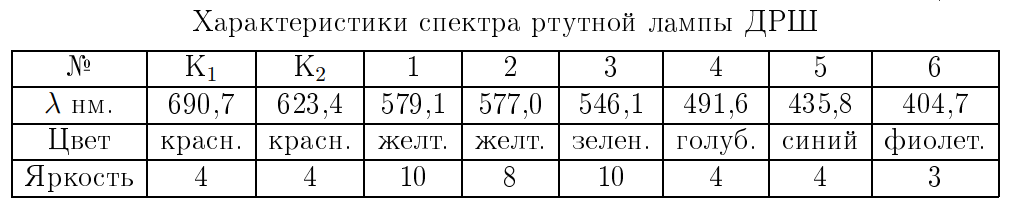
\includegraphics[width = 14cm]{2}}
	\label{fig:image}
\end{figure}

Теперь можем построить графики зависимости $\sin\varphi(\lambda)$:

\begin{flushleft}
\begin{tikzpicture}
\begin{axis}[
	height = 9cm,
	width  = 15cm,
	every axis y label/.style={at = {(ticklabel cs: 0.5)}, rotate = 90, anchor = near ticklabel},
	xlabel = {$\lambda$, нм},
	ylabel = {$\sin\varphi$},
	xtick  = {400,450,500,550,600,650,700},
	ytick  = {0.20,0.22,0.24,0.26,0.28,0.30,0.32},
	y tick label style={/pgf/number format/fixed zerofill}
]
\addplot+[%error bars/.cd, 
	%y dir = both, y explicit,
	%x dir = both, x explicit,
	only marks
	]
coordinates{
	(404.7, 0.20222)
	(435.8, 0.21928)
	(491.6, 0.24492)
	(546.1, 0.27284)
	(577.0, 0.28793)
	(579.1, 0.28923)
	(623.4, 0.30488)
	(690.7, 0.31129)
};

\addplot [mark = none]
coordinates{
	(400, 0.2005)
	(640, 0.320)
};

\end{axis}
\end{tikzpicture}
\end{flushleft}

\begin{flushleft}
\begin{tikzpicture}
\begin{axis}[
	height = 9cm,
	width  = 14.6cm,
	every axis y label/.style={at = {(ticklabel cs: 0.5)}, rotate = 90, anchor = near ticklabel},
	xlabel = {$\lambda$, нм},
	ylabel = {$\sin\varphi$},
	xtick  = {400,450,500,550,600,650,700},
	ytick  = {-0.20,-0.22,-0.24,-0.26,-0.28,-0.30,-0.32},
	y tick label style={/pgf/number format/fixed zerofill}
]
\addplot+[%error bars/.cd, 
	%y dir = both, y explicit,
	%x dir = both, x explicit,
	only marks
	]
coordinates{
	(404.7, -0.20257)
	(435.8, -0.21937)
	(491.6, -0.24576)
	(546.1, -0.27296)
	(577.0, -0.28893)
	(579.1, -0.29009)
	(623.4, -0.30488)
	(690.7, -0.31129)
};

\addplot [mark = none]
coordinates{
	(400, -0.2005)
	(640, -0.320)
};

\end{axis}
\end{tikzpicture}
\end{flushleft}

При измерениях будем отмечать угловую координату каждой из линий, описанных в ТО, не усредняя результата, для близких линий. В выбранном масштабе погрешность на графике будет незаметна.

\vspace{1cm}
Найдем угловые коэффициенты графиков:
$$
	k_1 = 494\cdot10^3\text{м}^{-1}
$$
$$
	k_2 = 498\cdot10^3\text{м}^{-1}
$$
Найдем случайную погрешность $k_1$ и $k_2$, используя МНК:
$$
	\sigma_{k_1 \text{случ}} = 11\cdot10^3\text{м}^{-1}
$$
$$
	\sigma_{k_6 \text{случ}} = 13\cdot10^3\text{м}^{-1}
$$
Приборная порешность при этом вычисляется из предположения, что $k = f(\varphi, \lambda)$:
$$
	\sigma_\text{приб} = \frac{\partial f}{\partial \varphi}\sigma_\varphi = \frac{\cos\varphi}{\lambda}\sigma_\varphi
$$
И заметно меньше случайной погрешности, в связи с чем ей можно пренебречь. Таким образом:
$$
	k_1 = (494 \pm 11)\cdot10^3\text{м}^{-1}
$$
$$
	k_2 = (498 \pm 13)\cdot10^3\text{м}^{-1}
$$
Откуда
$$
	d_1 = (202 \pm 5)\cdot10^{-8}\text{м}
$$
$$
	d_2 = (201 \pm 5)\cdot10^{-8}\text{м}
$$

\vspace{1cm}
Таким образом, получим:

\begin{center}
\boxed{$$d = (202 \pm 5)\cdot10^{-8}\text{м}$$}
\end{center}


Для оценки угловой дисперсии решётки определим угловые координаты линий жёлтой пары во всех видимых порядках спектра, положительных и отрицательных.

\begin{center}
\begin{tabular}{|c|c|c|c|c|c|c|c|c|c|c|c|c|c|}
\hline
$m$	&	$\varphi_1$	&	$\varphi_2$	&	$\Delta\varphi$	&	$D$, $^\circ/$\r{A}\\
\hline
-2	&	215'06'40	&	215'14'30	&	0'07'50			&	0.39				\\
\hline
-1	&	196'51'47	&	196'47'50	&	0'03'57			&	0.20				\\
\hline
1	&	163'16'54	&	163'13'03	&	0'03'51			&	0.19				\\
\hline
2	&	144'53'27	&	144'45'31	&	0'07'56			&	0.40				\\
\hline
\end{tabular}
\end{center}

Погрешности принимаем теми же, какие мы брали в предыдущем пункте. Найдем среднее значение длины волны: $(577.0+579.1)/2 = 578.1$нм, откуда, зная, что 
$$
	D = \frac{m}{\sqrt{d^2 - m^2\lambda^2}}
$$
получим:

\begin{flushleft}
\begin{tikzpicture}
\begin{axis}[
	height = 9cm,
	width  = 15cm,
	every axis y label/.style={at = {(ticklabel cs: 0.5)}, rotate = 90, anchor = near ticklabel},
	xlabel = {$m$},
	ylabel = {$D$, $^\circ/$\r{A}},
%	xtick  = {400,450,500,550,600,650,700},
%	ytick  = {0.20,0.22,0.24,0.26,0.28,0.30,0.32},
%	y tick label style={/pgf/number format/fixed zerofill}
]
\addplot+[%error bars/.cd, 
	%y dir = both, y explicit,
	%x dir = both, x explicit,
	only marks
	]
coordinates{
	(-2,-0.39)
	(-1,-0.20)
	( 1, 0.19)
	( 2, 0.40)
};

\addplot+[%error bars/.cd, 
	%y dir = both, y explicit,
	%x dir = both, x explicit,
	only marks,
	color = red
	]
coordinates{
	(-2,-0.40)
	(-1,-0.20)
	( 1, 0.20)
	( 2, 0.40)
};

\addplot [mark = none]
coordinates{
	(-2, -0.394)
	(2, 0.394)
};

\end{axis}
\end{tikzpicture}
\end{flushleft}


Для определения аппаратной разретающей способности (решётка + гониометр + глаз наблюдателя) измерим угловую ширину одной из линий желтой пары (по нулям интенсивности) в нескольких порядках. Предварительно установим минимальную ширину щели коллиматора, позволяющую вести измерения.

Для качественного определения аппаратной разрешающей способности $R$ оценим, во сколько раз расстояние между центрами жёлтых линий ($\Delta\lambda = 20$\r{A}) больше полуширины одной линии и рассчитаем аппаратную полуширину линии $\delta\lambda$:
$$
	R = \frac{\lambda}{\delta\lambda} = \frac{\varphi}{\delta\varphi}
$$ 

Считая погрешность угла равной $\sigma_\varphi = 0^\circ00'05"$, получим:

\begin{center}
\begin{tabular}{|c|c|c|c|c|c|c|c|c|c|c|c|c|c|}
\hline
$m$	&	$\varphi_1$	&	$\varphi_2$	&	$\Delta\varphi$	&	$R$		&	$\delta\lambda$, нм		&	$N$		&	$\sigma_N$	\\
\hline
1	&	163'08'24	&	163'07'34	&	0'00'50			&	1200	&	0.48					&	1200	&	200			\\
\hline
2	&	144'56'14	&	144'55'17	&	0'00'57			&	2200	&	0.26					&	1100	&	200			\\
\hline
\end{tabular}
\end{center}

\vspace{1cm}
\textbf{III. Зависимость разрешающей силы от ширины пучка}

Настроим зрительную трубу на жёлтую пару. Держа в руке дополнительную щель с микрометрическим винтом и рассматривая сквозь неё светящийся объект, определим начало отсчёта -- момент открытия щели. Трижды повторим процедуру определения нуля, каждый раз открывая щель все медленнее.

Откроем щель пошире и укрепим её на коллиматорном объективе. Уменьшая ширину щели, добьемся предельного разрешения жёлтой пары и запишем показания микрометрического винта щели. Зная разность длин волн для жёлтой пары, оценим разрешающую способность $R$ в этом эксперименте, число эффективно работающих штрихов $N$ по формуле $R = mN$ и число штрихов на мм.

Предельная ширина щели равна $1.2\pm0.1$мм. Погрешность оценим, немного меняя толщину щели и наблюдая за картинкой - в эти пределах она менялась несильно. Измерим углы, соответствующие минимумам левой и правой линии:

\begin{center}
\begin{tabular}{|c|c|c|c|c|c|c|c|c|c|c|c|c|c|}
\hline
$m$	&	$\varphi_1$	&	$\varphi_2$	&	$\varphi_3$	&	$\varphi_4$	\\
\hline
1	&	163'19'35	&	163'16'57	&	163'15'35	&	163'13'46	\\
\hline
\end{tabular}
\end{center}

Или же, найдя реальные значения углов:

\begin{center}
\begin{tabular}{|c|c|c|c|c|c|c|c|c|c|c|c|c|c|}
\hline
$m$	&	$\varphi_1$	&	$\varphi_2$	&	$\varphi_3$	&	$\varphi_4$	\\
\hline
1	&	16'40'25	&	16'43'03	&	16'44'25	&	16'46'14	\\
\hline
\end{tabular}
\end{center}

Из полученных значений оценим $R$ по формуле:
$$
	R = \frac{\varphi}{\delta\varphi} = \frac{(\varphi_1 + \varphi_4)/2}{(\varphi_4+\varphi_3)/2 - (\varphi_2+\varphi_1)/2} = 
	    \frac{\varphi_1 + \varphi_4}{\varphi_4+\varphi_3 - \varphi_1-\varphi_2}
$$

Откуда:
$$
	R = 300 \pm 30
$$

Теперь по формуле $R = mN$ можно найти $N$ и оценить число штрихов на миллиметр.
$$
	N = 300 \pm 30,
$$
$$
	n = N/l = 250 \pm 50
$$
\noindent где $l$ - толщина щели. Погрешность $n$ определим, считая $n = f(N, l)$. Величина $n$ не совпадает с номинальной в силу того, что на него влияет качество реплики, толщина источника и прочие факторы.

\newpage
Таким образом, в данной лабораторной работе мы исследовали дифракционную решетку, а также оценили разрешающую способность используемого в работе гониометра.


\end{document}